\appendix
\addcontentsline{toc}{section}{Appendici}
%\section*{Appendici}
\newsection{Resoconto delle attività di verifica}
Questa sezione riporta il resoconto delle attività di verifica svolte prima di ciascuna delle quattro revisioni stabilite dal committente (Revisione dei Requisiti, R. di Progettazione, R. di Qualifica e R. di Accettazione).
Al termine di ogni revisione il committente segnalerà le problematiche riscontrate attraverso una valutazione globale dell'andamento del progetto ed una dettagliata per ciascun documento, permettendo al gruppo di eliminare problemi e criticità nel progetto per poi procedere su una base verificata e il più possibile corretta.

\subsection{Revisione dei Requisiti}
In questa sezione vengono riportati gli esiti delle metriche relative ai processi e ai documenti durante la fase di Analisi.
\subsubsection{Qualità di processo}
\paragraph{Esiti metriche di processo} \MiniSpazio
\renewcommand{\arraystretch}{1.5}
\begin{table}[H]
	\begin{center}
		\begin{tabular}{|c|c|c|}
			\hline
			\rowcolor{title_row}
			\textbf{\color{title_text}{Metrica}} & \textbf{\color{title_text}{Valore ottenuto}} & \textbf{\color{title_text}{Esito}} \\
			\hline
			{Schedule Variance} & {0} & {Superato}\\	
			\hline
			{Budget Variance} & {-2.5\%} & {Superato}\\	
			\hline
		\end{tabular}
	\caption[Esiti metriche di processo, Analisi]{Esiti derivanti dall'applicazione delle metriche di processo}	
	\label{tabella: esiti derivanti dall'applicazione delle metriche di processo}
	\end{center}
\end{table}
\renewcommand{\arraystretch}{1}
\paragraph{Dettaglio delle verifiche tramite analisi} \Spazio
Il grafico rappresentante l'applicazione del metodo PDCA della fase di Analisi è:
\begin{figure} [H]
	\centering
	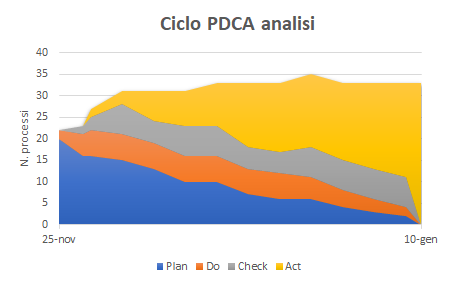
\includegraphics[scale=1]{Img/Ciclo_PDCA}
	\caption{Grafico del metodo PDCA, fase di Analisi}\label{immagine:pdca analisi}
\end{figure}
Dal grafico possiamo estrapolare che:
\begin{itemize}
	\item Alcuni dei processi pianificati hanno subito mutamenti, dovuti ad errori di pianificazione dati dalla poca esperienza del gruppo di lavoro;
	\item Il gruppo ha reso l'avanzamento dei processi omogeneo, nonostante alcuni rallentamenti dovuti alla sovrapposizione di impegni personali e universitari dei componenti del gruppo con la realizzazione del progetto. Nel complesso si vede come l'omogeneità è stata abbastanza rispettata.
\end{itemize}
\subsubsection{Qualità di prodotto}
\paragraph{Indice di Gulpease} \Spazio
Vengono qui riportati i valori dell'indice Gulpease per ogni documento durante la fase di Analisi. 
\renewcommand{\arraystretch}{1.5}
\begin{table}[H]
\begin{center}
\begin{tabular}{|c|c|c|}
\hline
\rowcolor{title_row}
\textbf{\color{title_text}{Documento}} & \textbf{\color{title_text}{Valore indice}} & \textbf{\color{title_text}{Esito}} \\
\hline
	\emph{Piano di Progetto v1.0.0} & {55.49} & {Superato}\\
\hline
	\emph{Norme di Progetto v1.0.0} & {54.54} & {Superato}\\
\hline
	\emph{Analisi dei Requisiti v1.0.0} & {58.80} & {Superato}\\
\hline
	\emph{Piano di Qualifica v1.0.0} & {53.98} & {Superato}\\
\hline
	\emph{Studio di Fattibilità v1.0.0} & {50.77} & {Superato}\\
\hline
	\emph{Glossario v1.0.0} & {51.66} & {Superato}\\
\hline
\end{tabular}
\caption[Esiti verifica documenti, Analisi]{Indice di Gulpease per documento, fase di Analisi}
\label{tabella:verifica documenti}
\end{center}
\end{table}
\renewcommand{\arraystretch}{1}

Dalla tabella si può notare come tutti gli indici Gulpease dei documenti rientrino nei vincoli dati. Per questo motivo i documenti redatti hanno raggiunto la leggibilità desiderata.

\subsubsection{Dettaglio dell'esito della revisione}
\begin{itemize}
	\item\emph{Norme di Progetto}: sono state effettuate le integrazioni richieste ed è stata aggiornata la struttura del documento in modo da rispettare gli stessi standard per ogni sezione;\\
	La sottosezione relativa alla verifica è stata aggiornata in modo da contenere le nuove metriche inserite e le metriche erroneamente inserite nel \emph{Piano di Qualità v1.0.0}.	\item\emph{Analisi dei Requisiti}: sono state attuate le opportune modifiche suggerite. Alcuni casi d'uso sono stati leggermente rivisti ed è stato introdotto un caso d'uso più generico per ogni agglomerato di azioni con attitudini simili, modificando il caso d'uso principale; 	
	\item\emph{Piano di Progetto}: sono state fatte alcune verifiche nell'uso di alcuni termini e standard come consigliato dal committente. Sono state aggiunte le opportune motivazioni e spiegazioni nelle scelte effettuate. La presentazione dei contenuti è stata rivista in modo da renderla più efficace;
	\item\emph{Piano di Qualifica}: il documento è stato profondamente rivisto per struttura e contenuti secondo quanto specificato dal committente.
	Le specifiche degli standard utilizzati e le descrizioni delle metriche sono stati spostati in appendice alle \emph{Norme di Progetto}. È stata aggiunta una sezione riguardante la pianificazione dei test, e le specifiche dei test sono state previste come futura aggiunta in appendice al documento. Infine, la strategia generale per la verifica ha assunto un ruolo centrale nella specifica degli obiettivi di qualità di processo e prodotto. 
\end{itemize}

\subsection{Revisione di Progettazione}
In questa sezione vengono riportati gli esiti delle metriche relative ai processi e delle metriche relative ai documenti.

\subsubsection{Qualità di processo}
\paragraph{Esiti metriche di processo}

\subparagraph{Consolidamento dei requisiti}\MiniSpazio
\renewcommand{\arraystretch}{1.5}
\begin{table}[H]
	\begin{center}
		\begin{tabular}{|c|c|c|}
			\hline
			\rowcolor{title_row}
			\textbf{\color{title_text}{Metrica}} & \textbf{\color{title_text}{Valore ottenuto}} & \textbf{\color{title_text}{Esito}} \\
			\hline
			{Schedule Variance} & {0} & {Superato}\\	
			\hline
			{Budget Variance} & {8\%} & {Superato}\\	
			\hline
		\end{tabular}
		\caption[Esiti metriche di processo, consolidamento dei requisiti]{Esiti derivanti dall'applicazione delle metriche di processo}	
		\label{tabella: esiti derivanti dall'applicazione delle metriche di processo cr}
	\end{center}
\end{table}


\subparagraph{Progettazione architetturale}\MiniSpazio
\renewcommand{\arraystretch}{1.5}
\begin{table}[H]
	\begin{center}
		\begin{tabular}{|c|c|c|}
			\hline
			\rowcolor{title_row}
			\textbf{\color{title_text}{Metrica}} & \textbf{\color{title_text}{Valore ottenuto}} & \textbf{\color{title_text}{Esito}} \\
			\hline
			{Schedule Variance} & {-3} & {Superato}\\	
			\hline	
			{Budget Variance} & {6\%} & {Superato}\\	
			\hline
			{Numero rischi non previsti} & {4} & {Superato}\\	
			\hline
			{Indisponibilità servizi esterni} & {0} & {Superato}\\	
			\hline
			{Media commit a settimana} & {26} & {Superato}\\	
			\hline
			{Media build Travis a settimana} & {22} & {Superato}\\	
			\hline
			{Percentuale build Travis superate} & {72.72\%} & {Superato}\\	
			\hline
		\end{tabular}
		\caption[Esiti metriche di processo, Progettazione Architetturale]{Esiti derivanti dall'applicazione delle metriche di processo}	
		\label{tabella: esiti derivanti dall'applicazione delle metriche di processo pa}
	\end{center}
\end{table}

\begin{figure} [H]
	\centering
	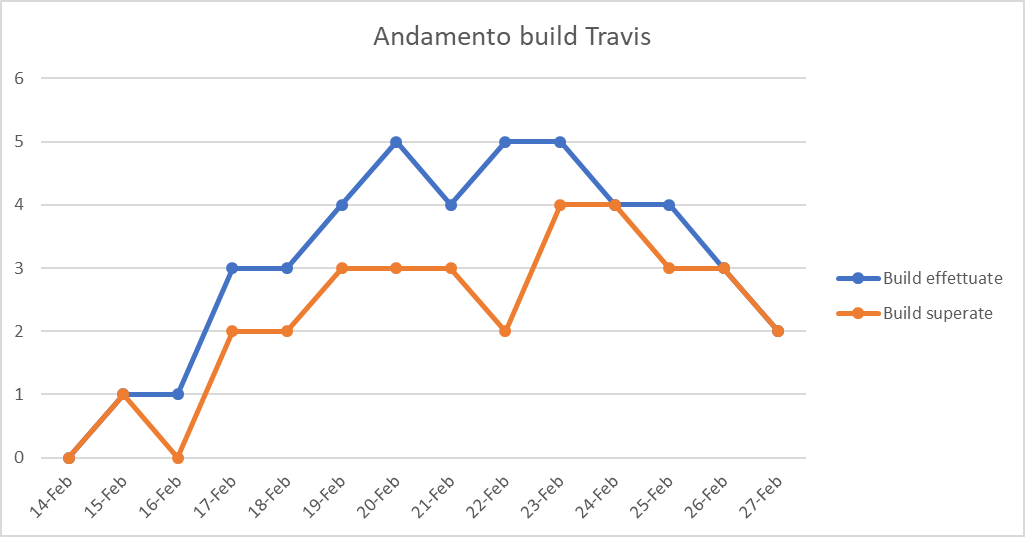
\includegraphics[scale=0.8]{Img/travis}
	\caption{Andamento delle build per il Proof of Concept}\label{}
\end{figure}

\paragraph{Maturità dei processi} \Spazio
Come riportato nella sezione 2.1.6, il gruppo adotta l'approccio a maturità di processo. Il livello di maturità assume valori da 1 a 5.

\subparagraph{Consolidamento dei requisiti}\MiniSpazio
\renewcommand{\arraystretch}{1.5}
\begin{table}[H]
	\begin{center}
		\begin{tabular}{|c|c|p{6.8cm}|}
			\hline
			\rowcolor{title_row}
			\textbf{\color{title_text}{Processo}} & \textbf{\color{title_text}{Livello di maturità}} & \textbf{\color{title_text}{Considerazioni}} \\
			\hline
			{Pianificazione e controllo} & {3} & {Gestito con l'ausilio di nTask, ha permesso di rispettare le scadenze previste.}\\	
			\hline
			{Gestione dei rischi} & {1} & {Non si sono verificate situazioni di rischio.}\\	
			\hline
			{Gestione dei test} & {0} & {Verrà istanziato una volta presente la necessità di definire e condurre dei test.}\\	
			\hline
			{Versionamento e build} & {0} & {Verrà istanziato una volta presente la necessità di versionare il prodotto software.}\\	
			\hline
		\end{tabular}
		\caption[Maturità dei processi, Consolidamento]{Maturità dei processi e considerazioni}	
		\label{tabella: considerazioni sulla maturità dei processi raggiunta}
	\end{center}
\end{table}
\pagebreak
\subparagraph{Progettazione architetturale}\MiniSpazio
\renewcommand{\arraystretch}{1.5}
\begin{table}[H]
	\begin{center}
		\begin{tabular}{|c|c|p{6.8cm}|}
			\hline
			\rowcolor{title_row}
			\textbf{\color{title_text}{Processo}} & \textbf{\color{title_text}{Livello di maturità}} & \textbf{\color{title_text}{Considerazioni}} \\
			\hline
			{Pianificazione e controllo} & {3} & {Ha permesso di rispettare le scadenze previste.}\\	
			\hline
			{Gestione dei rischi} & {1} & {Si è dimostrato poco stabile al verificarsi di 3 situazioni di rischio (malattia di membri del gruppo), comportando una ridefinizione degli obiettivi per il periodo.}\\	
			\hline
			{Gestione dei test} & {1} & {Sono stati pianificati i primi test di sistema, le cui specifiche tuttavia rimangono da definire.}\\	
			\hline
			{Versionamento e build} & {1} & {Parzialmente automatizzato con l'utilizzo dello strumento \gl{Travis}.}\\	
			\hline
		\end{tabular}
		\caption[Maturità dei processi, Progettazione Architetturale]{Maturità dei processi e considerazioni}	
		\label{tabella: considerazioni sulla maturità dei processi raggiunta pa}
	\end{center}
\end{table}
\renewcommand{\arraystretch}{1}

\paragraph{Dettaglio delle verifiche tramite analisi}
\subparagraph{Consolidamento dei requisiti}\MiniSpazio
Il grafico rappresentante l'applicazione del metodo PDCA nella fase di Consolidamento dei requisiti è:
\begin{figure} [H]
	\centering
	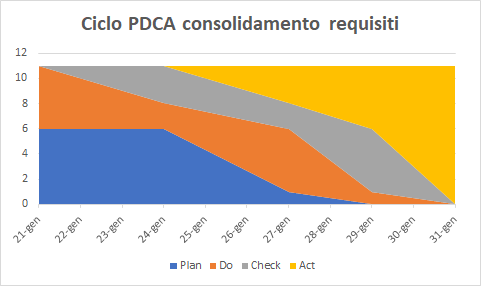
\includegraphics[scale=1]{Img/Ciclo_PDCA_consolidamento_requisiti}
	\caption{Grafico del metodo PDCA, fase di Consolidamento dei requisiti}\label{}
\end{figure}
Dal grafico possiamo estrapolare che:
\begin{itemize}
	\item Trattandosi di un periodo relativamente breve (10 giorni), piccole variazioni nel numero di attività risultano in grossi cambiamenti grafici;
	\item Le attività in Plan sono state esaurite prima del termine del periodo, mentre quelle in Check e Act hanno avuto una permanenza maggiore; ciò è dovuto ad un numero di modifiche ai documenti relativamente basso ma di grande importanza e profondità (soprattutto per quanto riguarda il consolidamento del \emph{Piano di Qualifica}), che quindi hanno richiesto periodi di Check e Act prolungati.
\end{itemize}
\subparagraph{Progettazione architetturale}\MiniSpazio
Il grafico rappresentante l'applicazione del metodo PDCA nella fase di Progettazione architetturale è:
\begin{figure} [H]
	\centering
	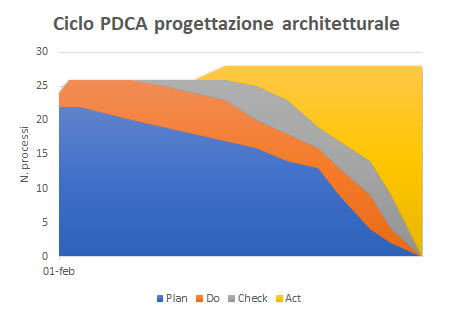
\includegraphics[scale=1]{Img/Ciclo_PDCA_progettazione_architetturale}
	\caption{Grafico del metodo PDCA, fase di Progettazione architetturale}\label{}
\end{figure}
Dal grafico possiamo estrapolare che:
\begin{itemize}
	\item Si nota uno stallo nell'esecuzione delle attività nella prima metà del periodo, dovuto principalmente, come previsto, alla sovrapposizione degli impegni universitari dei vari membri del gruppo. A questo si sono aggiunte le situazioni di rischio verificatesi, comportando ulteriori ritardi;
	\item Verso al fine del periodo si nota un rapido decremento delle attività in Do e Check, dovuto ad uno sforzo maggiorato per compensare i ritardi dovuti alle situazioni di rischio verificatesi.
\end{itemize}
\subsubsection{Qualità di prodotto}
\paragraph{Indice di Gulpease} \Spazio
Vengono qui riportati i valori dell'indice Gulpease per ogni documento al termine della fase di Progettazione Architetturale.
\renewcommand{\arraystretch}{1.5}
\begin{table}[H]
	\begin{center}
		\begin{tabular}{|c|c|c|}
			\hline
			\rowcolor{title_row}
			\textbf{\color{title_text}{Documento}} & \textbf{\color{title_text}{Valore indice}} & \textbf{\color{title_text}{Esito}} \\
			\hline
			\emph{Piano di Progetto v2.0.0} & {53.78} & {Superato}\\
			\hline
			\emph{Norme di Progetto v2.0.0} & {53.87} & {Superato}\\
			\hline
			\emph{Analisi dei Requisiti v2.0.0} & {59.02} & {Superato}\\
			\hline
			\emph{Piano di Qualifica v2.0.0} & {49.68} & {Superato}\\
			\hline
			\emph{Studio di Fattibilità v1.0.0} & {50.77} & {Superato}\\
			\hline
			\emph{Glossario v2.0.0} & {52.11} & {Superato}\\
			\hline
		\end{tabular}
		\caption[Esiti verifica documenti, Consolidamento e Progettazione Architetturale]{Indice di Gulpease per documento, fase di Progettazione Architetturale}
		\label{tabella:verifica documenti rp}
	\end{center}
\end{table}
\renewcommand{\arraystretch}{1}
Dalla tabella si può notare come tutti gli indici Gulpease dei documenti rientrino nei vincoli dati. Per questo motivo i documenti redatti hanno raggiunto la leggibilità desiderata.

\begin{figure} [H]
	\centering
	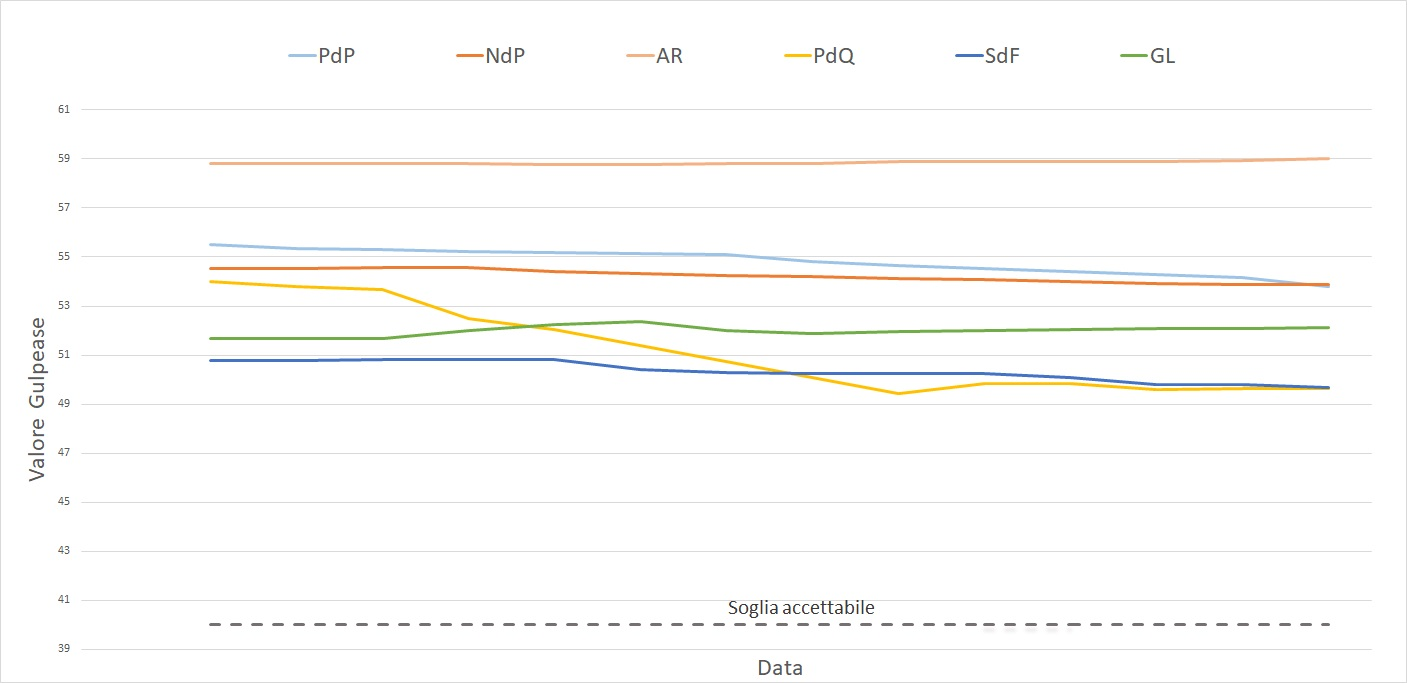
\includegraphics[scale=0.55]{Img/and_gulp_rp}
	\caption{Andamento dell'indice di Gulpease durante le fasi di Consolidamento dei requisiti e Progettazione architetturale}\label{immagine:gulpease rp}
\end{figure}

\pagebreak

\paragraph{Gunning fog index} \Spazio
\renewcommand{\arraystretch}{1.5}
\begin{table}[H]
	\begin{center}
		\begin{tabular}{|c|c|c|}
			\hline
			\rowcolor{title_row}
			\textbf{\color{title_text}{Documento}} & \textbf{\color{title_text}{Valore indice}} & \textbf{\color{title_text}{Esito}} \\
			\hline
			\emph{Piano di Progetto v2.0.0} & {13.21} & {Superato}\\
			\hline
			\emph{Norme di Progetto v2.0.0} & {12.74} & {Superato}\\
			\hline
			\emph{Analisi dei Requisiti v2.0.0} & {11.96} & {Superato}\\
			\hline
			\emph{Piano di Qualifica v2.0.0} & {12.87} & {Superato}\\
			\hline
			\emph{Studio di Fattibilità v1.0.0} & {11.18} & {Superato}\\
			\hline
			\emph{Glossario v2.0.0} & {14.39} & {Superato}\\
			\hline
		\end{tabular}
		\caption[Esiti verifica documenti, Consolidamento e Progettazione Architetturale]{Gunning fog index per documento, fase di Progettazione Architetturale}
		\label{tabella:verifica documenti gf}
	\end{center}
\end{table}
Dalla tabella si può notare come tutti gli indici Gunning fox dei documenti rientrino nei vincoli dati. Per questo motivo i documenti redatti hanno raggiunto la leggibilità desiderata.

\paragraph{Numero errori ortografici} \Spazio
Grazie le procedura di verifica e correzione attuate e all'ausilio dello strumento di controllo ortografico integrato in \gl{TexStudio}, il numero di errori ortografici per ogni documento ha raggiunto il valore ottimale di 0.

\newsection{Specifica dei test}
\subsection{Test di accettazione}
\normalsize
\renewcommand{\arraystretch}{1}
\begin{longtable}{|C{2.5cm}|C{13cm}|}
	\hline
	\rowcolor{title_row}
	\textbf{\color{title_text}{Test}} & \textbf{\color{title_text}{Specifica}}  \\
	\hline
	\endhead
{TA-1} &
\begin{itemize}
	\item \textbf{Progettazione}: verifica che il sistema permetta di leggere la definizione di una rete Bayesiana importando un file in formato JSON;
	\item \textbf{Caso}: 
		\begin{itemize}
			\item \textbf{Input}: file JSON con la definizione di rete;
			\item \textbf{Output}: il sistema importa la definizione della rete mostrandone il contenuto.
		\end{itemize}
	\item \textbf{Procedura}:
		\begin{itemize}
			\item L'utente crea un nuovo 7DOS panel;
			\item L'utente si posiziona sulla scheda di \emph{"Edit"};
			\item L'utente si posiziona sul \emph{"JSON import"} panel;
			\item L'utente preme il pulsante per importare un file JSON;
			\item L'utente seleziona il file da importare;
			\item Conferma la selezione del file.
		\end{itemize} 
\end{itemize} \\
\hline

{TA-2} &
\begin{itemize}
	\item \textbf{Progettazione}: verifica che il sistema permetta la gestione della connessione tra i nodi della rete ed il flusso di dati;
	\item \textbf{Caso}: 
	\begin{itemize}
		\item \textbf{Input}:
		\item \textbf{Output}: il sistema effettua la connessione tra flusso dati e nodi della rete.
	\end{itemize}
	\item \textbf{Procedura}:
	\begin{itemize}
		\item L'utente si posiziona sulla scheda di \emph{"Edit"};
		\item L'utente si posiziona sul \emph{"Network"} panel;
		\item L'utente seleziona il flusso di dati da monitorare.
	\end{itemize} 
\end{itemize} \\
 \hline
{TA-2.1} &
\begin{itemize}
	\item \textbf{Progettazione}: verifica che il sistema permetta di connettere un nodo della rete al flusso di dati;
	\item \textbf{Caso}: 
	\begin{itemize}
		\item \textbf{Input}: 
		\item \textbf{Output}: il sistema connette il nodo selezionato e lo monitora rispetto al flusso dati.
	\end{itemize}
	\item \textbf{Procedura}:
	\begin{itemize}
		\item L'utente si posiziona sulla scheda di \emph{"Edit"};
		\item L'utente si posiziona sul \emph{"Network"} panel;
		\item L'utente seleziona il nodo da monitorare rispetto al flusso di dati.
	\end{itemize} 
\end{itemize} \\
\hline
{TA-2.2} &
\begin{itemize}
	\item \textbf{Progettazione}: verifica che il sistema permetta di disconnettere un nodo della rete al flusso di dati;
	\item \textbf{Caso}: 
	\begin{itemize}
		\item \textbf{Input}:
		\item \textbf{Output}: il sistema disconnette il nodo selezionato.
	\end{itemize}
	\item \textbf{Procedura}:
	\begin{itemize}
		\item L'utente si posiziona sulla scheda di \emph{"Edit"};
		\item L'utente si posiziona sul \emph{"Network"} panel;
		\item L'utente deseleziona il nodo da monitorare rispetto al flusso di dati.
	\end{itemize} 
\end{itemize} \\
\hline
{TA-2.3} &
\begin{itemize}
	\item \textbf{Progettazione}: verifica che il sistema permetta di modificare un nodo della rete connesso al flusso di dati;
	\item \textbf{Caso}: 
	\begin{itemize}
		\item \textbf{Input}: 
		\item \textbf{Output}: il sistema apporta le modifiche richieste.
	\end{itemize}
	\item \textbf{Procedura}:
	\begin{itemize}
		\item L'utente si posiziona sulla scheda di \emph{"Edit"};
		\item L'utente si posiziona sul \emph{"Network"} panel;
		\item L'utente modifica il nodo da monitorare rispetto al flusso di dati.
	\end{itemize} 
\end{itemize}\\
\hline
{TA-3} &
\begin{itemize}
	\item \textbf{Progettazione}: verifica che il sistema permetta di applicare il
	ricalcolo delle probabilità della rete
	secondo regole temporali stabilite dall'utente.;
	\item \textbf{Caso}: 
	\begin{itemize}
		\item \textbf{Input}: 
		\item \textbf{Output}: il sistema effettua il ricalcolo delle probabilità della rete aggiornandone lo stato dei nodi.
	\end{itemize}
	\item \textbf{Procedura}:
	\begin{itemize}
		\item Il sistema legge i dati provenienti dal flusso;
		\item Il sistema li elabora calcolando le probabilità dei nodi;
		\item Il sistema aggiorna lo stato dei nodi.
	\end{itemize} 
\end{itemize}\\
\hline
{TA-3.1} &
\begin{itemize}
	\item \textbf{Progettazione}: verifica che il sistema permetta all'utente di modificare le regole temporali per effettuare il ricalcolo delle probabilità della rete;
	\item \textbf{Caso}: 
	\begin{itemize}
		\item \textbf{Input}: 
		\item \textbf{Output}: il sistema apporta le modifiche richieste alle regole temporali per il ricalcolo delle probabilità.
	\end{itemize}
	\item \textbf{Procedura}:
	\begin{itemize}
		\item L'utente si posiziona sulla scheda di \emph{"Edit"};
		\item L'utente si posiziona sul \emph{"Network"} panel;
		\item L'utente modifica le regole temporali per il ricalcolo delle probabilità della rete.
	\end{itemize} 
\end{itemize} \\
\hline
{TA-4} &
\begin{itemize}
	\item \textbf{Progettazione}: verifica che il sistema permetta fornire nuovi dati a Grafana derivati dai nodi
	della rete non direttamente collegati al flusso di
	dati;
	\item \textbf{Caso}: 
	\begin{itemize}
		\item \textbf{Input}: ;
		\item \textbf{Output}: .
	\end{itemize}
	\item \textbf{Procedura}:
	\begin{itemize}
		\item ;
		\item ;
		\item .
	\end{itemize} 
\end{itemize}\\
\hline
{TA-4.1} &
\begin{itemize}
	\item \textbf{Progettazione}: verifica che il sistema permetta l'aggiornamento dei dati secondo una frequenza stabilita dall'utente;
	\item \textbf{Caso}: 
	\begin{itemize}
		\item \textbf{Input}: ;
		\item \textbf{Output}: .
	\end{itemize}
	\item \textbf{Procedura}:
	\begin{itemize}
		\item ;
		\item ;
		\item .
	\end{itemize} 
\end{itemize} \\
\hline
{TA-5} &
\begin{itemize}
	\item \textbf{Progettazione}: verifica che il sistema permetta di leggere i dati provenienti dal flusso ed elaborarli, visualizzandone il risultato attraverso un grafico;
	\item \textbf{Caso}: 
	\begin{itemize}
		\item \textbf{Input}: flusso di dati;
		\item \textbf{Output}: grafico derivato dall'elaborazione dei dati.
	\end{itemize}
	\item \textbf{Procedura}:
	\begin{itemize}
		\item Il sistema legge i dati in ingresso dal flusso;
		\item Il sistema elabora i dati ricevuti;
		\item Il sistema costruisce un grafico sulla base dei risultati ottenuti.
	\end{itemize} 
\end{itemize} \\
\hline

{TA-5.1} &
\begin{itemize}
	\item \textbf{Progettazione}: verifica che il sistema aggiorni i dati presenti nel grafico in base alla frequenza stabilita dall'utente;
	\item \textbf{Caso}: 
	\begin{itemize}
		\item \textbf{Input}: nuovi dati dal flusso;
		\item \textbf{Output}: il sistema aggiorna i dati nel grafico.
	\end{itemize}
	\item \textbf{Procedura}:
	\begin{itemize}
		\item Il sistema legge i nuovi dati proveniente dal flusso, in base alla frequenza stabilita;
		\item Il sistema effettua il ricalcolo delle probabilità della rete aggiornando lo stato dei nodi, in base alla frequenza stabilita;
		\item Il sistema elabora i risultati e li mostra attraverso un grafico.
	\end{itemize} 
\end{itemize} \\
\hline
{TA-5.2} &
\begin{itemize}
	\item \textbf{Progettazione}: verifica che il sistema permetta all'utente di creare un nuovo panel;
	\item \textbf{Caso}: 
	\begin{itemize}
		\item \textbf{Input}:
		\item \textbf{Output}: il sistema crea il nuovo panel e lo mostra all'interno della dashboard..
	\end{itemize}
	\item \textbf{Procedura}:
	\begin{itemize}
		\item L'utente si posiziona all'interno di una dashboard;
		\item L'utente clicca sulla voce \emph{add panel};
		\item L'utente sceglie la tipologia di panel da creare.
	\end{itemize} 
\end{itemize} \\
\hline
{TA-5.3} &
\begin{itemize}
	\item \textbf{Progettazione}: verifica che il sistema permetta all'utente di spostare un panel all'interno della dashboard;
	\item \textbf{Caso}: 
	\begin{itemize}
		\item \textbf{Input}:
		\item \textbf{Output}: il sistema sposta panel nella nuova posizione scelta dall'utente.
	\end{itemize}
	\item \textbf{Procedura}:
	\begin{itemize}
		\item L'utente si posiziona all'interno di una dashboard;
		\item L'utente trascina il panel che vuole spostare nella posizione desiderata.
	\end{itemize} 
\end{itemize} \\
\hline
{TA-5.4} &
\begin{itemize}
	\item \textbf{Progettazione}: verifica che il sistema permetta all'utente di cancellare un panel all'interno della dashboard;
	\item \textbf{Caso}: 
	\begin{itemize}
		\item \textbf{Input}: ;
		\item \textbf{Output}: il sistema cancella panel scelto dall'utente.
	\end{itemize}
	\item \textbf{Procedura}:
	\begin{itemize}
		\item L'utente si posiziona all'interno di una dashboard;
		\item L'utente clicca sull'intestazione del panel;
		\item L'utente seleziona la voce \emph{"Remove"};
		\item Conferma l'eliminazione del panel.
	\end{itemize} 
\end{itemize} \\
\hline
{TA-5.5} &
\begin{itemize}
	\item \textbf{Progettazione}: verifica che il sistema permetta all'utente di minimizzare un panel;
	\item \textbf{Caso}: 
	\begin{itemize}
		\item \textbf{Input}: ;
		\item \textbf{Output}: il sistema modifica la dimensione del panel come scelto dall'utente.
	\end{itemize}
	\item \textbf{Procedura}:
	\begin{itemize}
		\item L'utente si posiziona all'interno di una dashboard;
		\item L'utente si posiziona sull'angolo in basso a destra del panel;
		\item L'utente modifica minimizza il panel.
	\end{itemize} 
\end{itemize} \\
\hline
{TA-5.6} &
\begin{itemize}
	\item \textbf{Progettazione}: verifica che il sistema permetta all'utente configurare un panel dopo la sua creazione;
	\item \textbf{Caso}: 
	\begin{itemize}
		\item \textbf{Input}: ;
		\item \textbf{Output}: il sistema configura le opzioni del panel come stabilito dall'utente.
	\end{itemize}
	\item \textbf{Procedura}:
	\begin{itemize}
		\item L'utente si posiziona all'interno di una dashboard;
		\item L'utente configura le opzioni del panel come desidera.
	\end{itemize} 
\end{itemize} \\
\hline
{TA-5.7} &
\begin{itemize}
	\item \textbf{Progettazione}: verifica che il sistema permetta all'utente di modificare un panel all'interno della dashboard;
	\item \textbf{Caso}: 
	\begin{itemize}
		\item \textbf{Input}: ;
		\item \textbf{Output}: il sistema modifica le opzioni del panel come stabilito dall'utente.
	\end{itemize}
	\item \textbf{Procedura}:
	\begin{itemize}
		\item L'utente si posiziona all'interno di una dashboard;
		\item L'utente modifica le opzioni del panel come desidera.
	\end{itemize} 
\end{itemize} \\
\hline
{TA-6} &
\begin{itemize}
	\item \textbf{Progettazione}: verifica che il sistema permetta all'utente di definire alert in base a livelli di soglia raggiunti dai nodi non collegati al flusso dei dati;
	\item \textbf{Caso}: 
	\begin{itemize}
		\item \textbf{Input}: ;
		\item \textbf{Output}: il sistema crea un nuovo alert.
	\end{itemize}
	\item \textbf{Procedura}:
	\begin{itemize}
		\item L'utente si posiziona all'interno di un panel di tipo \emph{graph};
		\item L'utente si posiziona sulla schermata di \emph{edit};
		\item L'utente si posiziona sulla scheda \emph{"Alert"};
		\item L'utente clicca sul pulsante \emph{"Create alert"}.
	\end{itemize} 
\end{itemize} \\
\hline
{TA-6.1} &
\begin{itemize}
	\item \textbf{Progettazione}: verifica che il sistema permetta all'utente di configurare i parametri di un alert;
	\item \textbf{Caso}: 
	\begin{itemize}
		\item \textbf{Input}: ;
		\item \textbf{Output}: il sistema configura i parametri dell'alert.
	\end{itemize}
	\item \textbf{Procedura}:
	\begin{itemize}
		\item L'utente si posiziona sulla scheda \emph{"Alert"};
		\item L'utente seleziona l'alert da configurare;
		\item L'utente configura i parametri come desidera.
	\end{itemize} 
\end{itemize} \\
\hline
{TA-6.2} &
\begin{itemize}
	\item \textbf{Progettazione}: verifica che il sistema permetta all'utente di impostare il modo in cui viene notificata l'attivazione di un alert;
	\item \textbf{Caso}: 
	\begin{itemize}
		\item \textbf{Input}: ;
		\item \textbf{Output}: il sistema imposta il sistema di notifica dell'alert.
	\end{itemize}
	\item \textbf{Procedura}:
	\begin{itemize}
		\item L'utente si posiziona sulla scheda \emph{"Alert"};
		\item L'utente seleziona l'alert da configurare;
		\item L'utente imposta come deve venire notificata l'attivazione dell'alert. 
	\end{itemize} 
\end{itemize} \\
\hline
{TA-7} &
\begin{itemize}
	\item \textbf{Progettazione}: verifica che il sistema permetta di disegnare una rete Bayesiana con un editor grafico specializzato;
	\item \textbf{Caso}: 
	\begin{itemize}
		\item \textbf{Input}: ;
		\item \textbf{Output}: .
	\end{itemize}
	\item \textbf{Procedura}:
	\begin{itemize}
		\item ;
	\end{itemize} 
\end{itemize} \\
\hline
{TA-7.1} &
\begin{itemize}
	\item \textbf{Progettazione}: verifica che il sistema permetta di creare un nuovo nodo della rete;
	\item \textbf{Caso}: 
	\begin{itemize}
		\item \textbf{Input}: ;
		\item \textbf{Output}: .
	\end{itemize}
	\item \textbf{Procedura}:
	\begin{itemize}
		\item ;
	\end{itemize} 
\end{itemize} \\
\hline
{TA-7.2} &
\begin{itemize}
	\item \textbf{Progettazione}: verifica che il sistema permetta di modificare i parametri di un nodo della rete;
	\item \textbf{Caso}: 
	\begin{itemize}
		\item \textbf{Input}: ;
		\item \textbf{Output}: .
	\end{itemize}
	\item \textbf{Procedura}:
	\begin{itemize}
		\item ;
	\end{itemize} 
\end{itemize} \\
\hline
{TA-7.3} &
\begin{itemize}
	\item \textbf{Progettazione}: verifica che il sistema permetta di creare un collegamento tra due nodi della rete;
	\item \textbf{Caso}: 
	\begin{itemize}
		\item \textbf{Input}: ;
		\item \textbf{Output}: .
	\end{itemize}
	\item \textbf{Procedura}:
	\begin{itemize}
		\item ;
	\end{itemize} 
\end{itemize} \\
\hline
{TA-7.4} &
\begin{itemize}
	\item \textbf{Progettazione}: verifica che il sistema permetta di eliminare un collegamento tra due nodi della rete;
	\item \textbf{Caso}: 
	\begin{itemize}
		\item \textbf{Input}: ;
		\item \textbf{Output}: .
	\end{itemize}
	\item \textbf{Procedura}:
	\begin{itemize}
		\item ;
	\end{itemize} 
\end{itemize}\\
\hline
{TA-7.5} &
\begin{itemize}
	\item \textbf{Progettazione}: verifica che il sistema permetta di salvare la rete realizzata su un file JSON;
	\item \textbf{Caso}: 
	\begin{itemize}
		\item \textbf{Input}: ;
		\item \textbf{Output}: .
	\end{itemize}
	\item \textbf{Procedura}:
	\begin{itemize}
		\item ;
	\end{itemize} 
\end{itemize} \\
\hline
{TA-7.6} &
\begin{itemize}
	\item \textbf{Progettazione}: verifica che il sistema rilevi e sia in grado di gestire eventuali errori derivati dalla modifica di un nodo;
	\item \textbf{Caso}: 
	\begin{itemize}
		\item \textbf{Input}: ;
		\item \textbf{Output}: .
	\end{itemize}
	\item \textbf{Procedura}:
	\begin{itemize}
		\item ;
	\end{itemize} 
\end{itemize} \\
\hline
{TA-8} &
\begin{itemize}
	\item \textbf{Progettazione}: verifica che il sistema permetta di applicare più reti Bayesiane a diversi oggetti di monitoraggio;
	\item \textbf{Caso}: 
	\begin{itemize}
		\item \textbf{Input}: ;
		\item \textbf{Output}: .
	\end{itemize}
	\item \textbf{Procedura}:
	\begin{itemize}
		\item ;
	\end{itemize} 
\end{itemize} \\
\hline
{TA-9} &
\begin{itemize}
	\item \textbf{Progettazione}: verifica che il sistema permetta di creare una rete Bayesiana a partire dai dati raccolti
	sul campo;
	\item \textbf{Caso}: 
	\begin{itemize}
		\item \textbf{Input}: ;
		\item \textbf{Output}: .
	\end{itemize}
	\item \textbf{Procedura}:
	\begin{itemize}
		\item ;
	\end{itemize} 
\end{itemize} \\
\hline
{TA-10} &
\begin{itemize}
	\item \textbf{Progettazione}: verifica che il sistema permetta di condividere grafici presenti in una dashboard o in un singolo panel;
	\item \textbf{Caso}: 
	\begin{itemize}
		\item \textbf{Input}: ;
		\item \textbf{Output}: il sistema condivide il grafico secondo l'opzione scelta dall'utente.
	\end{itemize}
	\item \textbf{Procedura}:
	\begin{itemize}
		\item L'utente si posiziona all'interno di una dashboard;
		\item L'utente seleziona l'opzione \emph{"Share"} relativa alla dashboard o ad un panel.
	\end{itemize} 
\end{itemize}\\
\hline
{TA-10.1} &
\begin{itemize}
	\item \textbf{Progettazione}: verifica che il sistema permetta di visualizzare il link diretto ad una dashboard o ad un
	panel;
	\item \textbf{Caso}: 
	\begin{itemize}
		\item \textbf{Input}: ;
		\item \textbf{Output}: il sistema mostra il link generato con cui l'utente può effettuare la condivisione.
	\end{itemize}
	\item \textbf{Procedura}:
	\begin{itemize}
		\item L'utente si posiziona all'interno di una dashboard;
		\item L'utente seleziona l'opzione \emph{"Share"} relativa alla dashboard o ad un panel;
		\item L'utente si posiziona sulla scheda \emph{"Link"};
		\item L'utente configura le opzioni per generare il link per la condivisione.
	\end{itemize} 
\end{itemize}\\
\hline
{TA-10.2} &
\begin{itemize}
	\item \textbf{Progettazione}: verifica che il sistema permetta di visualizzare il codice per l'inclusione di un panel in una pagina web;
	\item \textbf{Caso}: 
	\begin{itemize}
		\item \textbf{Input}: ;
		\item \textbf{Output}: Il sistema mostra il frame generato con cui l'utente può effettuare la condivisione.
	\end{itemize}
	\item \textbf{Procedura}:
	\begin{itemize}
		\item L'utente si posiziona all'interno di una dashboard;
		\item L'utente seleziona l'opzione \emph{"Share"} relativa ad un panel;
		\item L'utente si posiziona sulla scheda \emph{"Embed"};
		\item L'utente configura le opzioni per generare il frame per la condivisione.
	\end{itemize} 
\end{itemize}\\
\hline
{TA-10.4} &
\begin{itemize}
	\item \textbf{Progettazione}: verifica che il sistema permetta di condividere lo snapshot di una dashboard o di un
	panel;
	\item \textbf{Caso}: 
	\begin{itemize}
		\item \textbf{Input}: ;
		\item \textbf{Output}: il sistema effettua la condivisione dello snapshot.
	\end{itemize}
	\item \textbf{Procedura}:
	\begin{itemize}
		\item L'utente si posiziona all'interno di una dashboard;
		\item L'utente seleziona l'opzione \emph{"Share"} relativa a una dashboard ad un panel;
		\item L'utente si posiziona sulla scheda \emph{"Snapshot"};
		\item L'utente configura le opzioni per la condivisione dello snapshot.
	\end{itemize} 
\end{itemize}\\
\hline
{TA-10.5} &
\begin{itemize}
	\item \textbf{Progettazione}: verifica che il sistema permetta di visualizzare il codice JSON contenente la definizione
	di una dashboard;
	\item \textbf{Caso}: 
	\begin{itemize}
		\item \textbf{Input}: ;
		\item \textbf{Output}: il sistema mostra il codice JSON con la definizione della dashboard.
	\end{itemize}
	\item \textbf{Procedura}:
	\begin{itemize}
		\item L'utente si posiziona all'interno di una dashboard;
		\item L'utente seleziona l'opzione \emph{"Share dashboard"};
		\item L'utente si posiziona sulla scheda \emph{"Export"};
		\item L'utente clicca sul pulsante per visualizzare il JSON.
	\end{itemize} 
\end{itemize}\\
\hline
{TA-10.6} &
\begin{itemize}
	\item \textbf{Progettazione}: verifica che il sistema permetta di salvare il file JSON contenente la definizione di una
	dashboard;
	\item \textbf{Caso}: 
	\begin{itemize}
		\item \textbf{Input}: ;
		\item \textbf{Output}: il sistema effettua il salvataggio del codice JSON con la definizione della dashboard.
	\end{itemize}
	\item \textbf{Procedura}:
	\begin{itemize}
		\item L'utente si posiziona all'interno di una dashboard;
		\item L'utente seleziona l'opzione \emph{"Share dashboard"};
		\item L'utente si posiziona sulla scheda \emph{"Export"};
		\item L'utente clicca sul pulsante per salvare il JSON.
	\end{itemize} 
\end{itemize}\\
\hline
\caption{Specifica test di accettazione}
\end{longtable}
\renewcommand{\arraystretch}{1}
\newpage

\subsection{Test di sistema}
\normalsize
\renewcommand{\arraystretch}{1}
\begin{longtable}{|C{2.5cm}|C{13cm}|}
	\hline
	\rowcolor{title_row}
	\textbf{\color{title_text}{Test}} & \textbf{\color{title_text}{Specifica}}  \\
	\hline
	\endhead
	{TS-1} &
\begin{itemize}
	\item \textbf{Progettazione}: verifica che sia possibile e leggere la
	definizione della rete Bayesiana da un file in formato JSON;
	\item \textbf{Caso}: 
	\begin{itemize}
		\item \textbf{Input}: file JSON con la definizione di una rete Bayesiana;
		\item \textbf{Output}: il sistema legge il JSON e costruisce la rete.
	\end{itemize}
	\item \textbf{Procedura}:
	\begin{itemize}
		\item L'utente preme il pulsante per importare un file;
		\item L'utente seleziona il file;
		\item L'utente conferma la selezione.
	\end{itemize} 
\end{itemize} \\
	\hline
	{TS-1.1} &
\begin{itemize}
	\item \textbf{Progettazione}: verifica che sia possibile validare un
	file JSON;
	\item \textbf{Caso}: 
	\begin{itemize}
		\item \textbf{Input}: file JSON;
		\item \textbf{Output}: il sistema mostra degli errori se il file non è valido.
	\end{itemize}
	\item \textbf{Procedura}:
	\begin{itemize}
		\item L'utente seleziona un JSON da importare;
		\item L'utente conferma la selezione;
		\item Il sistema verifica la validità del file.
	\end{itemize} 
\end{itemize}\\
	\hline
	{TS-2} & 
\begin{itemize}
	\item \textbf{Progettazione}: verifica che sia possibile gestire la
	connessione tra i nodi della rete ai rispettivi flussi di dati;
	\item \textbf{Caso}: 
	\begin{itemize}
		\item \textbf{Input}: ;
		\item \textbf{Output}: il sistema effettua la connessione tra flusso dati e nodi della rete.
	\end{itemize}
	\item \textbf{Procedura}:
	\begin{itemize}
		\item L'utente si posiziona sul \emph{"Network"} panel;
		\item L'utente seleziona il flusso dati da monitorare.
	\end{itemize} 
\end{itemize} \\
	\hline
	{TS-2.1} &
\begin{itemize}
	\item \textbf{Progettazione}: verifica che sia possibile connettere un
	nodo della rete ad un flusso di dati;
	\item \textbf{Caso}: 
	\begin{itemize}
		\item \textbf{Input}: ;
		\item \textbf{Output}: il sistema connette il nodo selezionato al flusso dati.
	\end{itemize}
	\item \textbf{Procedura}:
	\begin{itemize}
		\item L'utente si posiziona sul \emph{"Network"} panel;
		\item L'utente sceglie quale nodo monitorare rispetto al flusso dati.
	\end{itemize} 
\end{itemize}	
	 \\
	\hline
	{TS-2.2} &
\begin{itemize}
	\item \textbf{Progettazione}: verifica che sia possibile disconnettere un
	nodo della rete da un flusso di dati.;
	\item \textbf{Caso}: 
	\begin{itemize}
		\item \textbf{Input}: ;
		\item \textbf{Output}: il sistema disconnette il nodo selezionato dal flusso dati.
	\end{itemize}
	\item \textbf{Procedura}:
	\begin{itemize}
		\item L'utente si posiziona sul \emph{"Network"} panel;
		\item L'utente sceglie quale nodo disconnettere rispetto al flusso dati.
	\end{itemize} 
\end{itemize}
	 \\
	\hline
	{TS-2.3} &
\begin{itemize}
	\item \textbf{Progettazione}: verifica che sia essere possibile modificare il
	flusso di dati connesso ad un nodo;
	\item \textbf{Caso}: 
	\begin{itemize}
		\item \textbf{Input}: ;
		\item \textbf{Output}: il sistema  seleziona un altro flusso di dati da associare alla rete.
	\end{itemize}
	\item \textbf{Procedura}:
	\begin{itemize}
		\item L'utente si posiziona sul \emph{"Network"} panel;
		\item L'utente modifica la fonte del flusso dati.
	\end{itemize} 
\end{itemize}	
	  \\
	\hline
	{TS-3} & 
\begin{itemize}
	\item \textbf{Progettazione}: verifica che sia possibile applicare il
	ricalcolo delle probabilità della rete secondo regole temporali prestabilite;
	\item \textbf{Caso}: 
	\begin{itemize}
		\item \textbf{Input}: flusso di dati;
		\item \textbf{Output}: il sistema effettua il ricalcolo delle probabilità della
		rete aggiornandone lo stato dei nodi.
	\end{itemize}
	\item \textbf{Procedura}:
	\begin{itemize}
		\item Il sistema legge i dati provenienti dal flusso;
		\item Il sistema li elabora calcolando le probabilità dei nodi;
		\item Il sistema aggiorna lo stato dei nodi.
	\end{itemize} 
\end{itemize}	
	\\
	\hline
	{TS-3.1} & 
\begin{itemize}
	\item \textbf{Progettazione}: verifica che sia possibile modificare le
	suddette regole temporali;
	\item \textbf{Caso}: 
	\begin{itemize}
		\item \textbf{Input}: ;
		\item \textbf{Output}: il sistema apporta le modifiche richieste alle regole temporali per il ricalcolo delle probabilità.
	\end{itemize}
	\item \textbf{Procedura}:
	\begin{itemize}
		\item L'utente si posiziona sulla scheda di \emph{"Edit"};
		\item L'utente si posiziona sul \emph{"Network"} panel;
		\item L'utente modifica le regole temporali per il ricalcolo delle probabilità della rete.
	\end{itemize} 
\end{itemize}
\\
	\hline
	{TS-4} & 
\begin{itemize}
	\item \textbf{Progettazione}: verifica che sia possibile fornire nuovi dati
	al sistema di Grafana derivati dai nodi della rete non collegati al flusso di
	monitoraggio;
	\item \textbf{Caso}: 
	\begin{itemize}
		\item \textbf{Input}: ;
		\item \textbf{Output}: .
	\end{itemize}
	\item \textbf{Procedura}:
	\begin{itemize}
		\item ;
		\item .
	\end{itemize} 
\end{itemize}
	\\
	\hline
	{TS-4.1} & 
\begin{itemize}
	\item \textbf{Progettazione}: verifica che sia possibile aggiornare i dati
	in base alla frequenza stabilita;
	\item \textbf{Caso}: 
	\begin{itemize}
		\item \textbf{Input}: ;
		\item \textbf{Output}: .
	\end{itemize}
	\item \textbf{Procedura}:
	\begin{itemize}
		\item ;
		\item .
	\end{itemize} 
\end{itemize}
	\\
	\hline
	{TS-5} & 
\begin{itemize}
	\item \textbf{Progettazione}: verifica che i dati siano disponibili al sistema di
	creazione di grafici e dashboard per la loro visualizzazione;
	\item \textbf{Caso}: 
	\begin{itemize}
		\item \textbf{Input}: flusso di dati;
		\item \textbf{Output}: grafico derivato dall'elaborazione dei dati.
	\end{itemize}
	\item \textbf{Procedura}:
	\begin{itemize}
		\item Il sistema legge i dati in ingresso dal flusso;
		\item Il sistema elabora i dati ricevuti;
		\item Il sistema costruisce un grafico sulla base dei risultati ottenuti.
	\end{itemize} 
\end{itemize}
	\\
	\hline
	{TS-5.1} & 
\begin{itemize}
	\item \textbf{Progettazione}: verifica che sia possibile aggiornare la
	dashboard in base alla frequenza stabilita;
	\item \textbf{Caso}: 
	\begin{itemize}
		\item \textbf{Input}: nuovi dati dal flusso;
		\item \textbf{Output}: il sistema aggiorna i dati nel grafico.
	\end{itemize}
	\item \textbf{Procedura}:
	\begin{itemize}
		\item Il sistema legge i nuovi dati proveniente dal flusso, in base alla frequenza stabilita;
		\item Il sistema effettua il ricalcolo delle probabilità della rete aggiornando lo stato dei nodi, in base alla frequenza stabilita;
		\item Il sistema elabora i risultati e li mostra attraverso un grafico.
	\end{itemize} 
\end{itemize}
\\
	\hline
	{TS-5.2} & 
\begin{itemize}
	\item \textbf{Progettazione}: verifica che sia possibile creare un panel;
	\item \textbf{Caso}: 
	\begin{itemize}
		\item \textbf{Input}: ;
		\item \textbf{Output}: il sistema crea il nuovo panel e lo mostra all'interno della dashboard.
	\end{itemize}
	\item \textbf{Procedura}:
	\begin{itemize}
		\item L'utente si posiziona all'interno di una dashboard;
		\item L'utente clicca sulla voce \emph{add panel};
		\item L'utente sceglie la tipologia di panel da creare.
	\end{itemize} 
\end{itemize}
 \\
	\hline
	{TS-5.3} & 
\begin{itemize}
	\item \textbf{Progettazione}: verifica che sia possibile spostare un panel;
	\item \textbf{Caso}: 
	\begin{itemize}
		\item \textbf{Input}: ;
		\item \textbf{Output}: il sistema sposta panel nella nuova posizione scelta dall'utente.
	\end{itemize}
	\item \textbf{Procedura}:
	\begin{itemize}
		\item L'utente si posiziona all'interno di una dashboard;
		\item L'utente trascina il panel che vuole spostare nella posizione desiderata.
	\end{itemize} 
\end{itemize}
	 \\
	\hline
	{TS-5.4} & 
\begin{itemize}
	\item \textbf{Progettazione}: verifica che sia possibile cancellare un
	panel;
	\item \textbf{Caso}: 
	\begin{itemize}
		\item \textbf{Input}: ;
		\item \textbf{Output}: il sistema cancella panel scelto dall'utente.
	\end{itemize}
	\item \textbf{Procedura}:
	\begin{itemize}
		\item L'utente si posiziona all'interno di una dashboard;
		\item L'utente clicca sull'intestazione del panel;
		\item L'utente seleziona la voce \emph{"Remove"};
		\item Conferma l'eliminazione del panel.
	\end{itemize} 
\end{itemize}
	 \\
	\hline
	{TS-5.5} & 
\begin{itemize}
	\item \textbf{Progettazione}: verifica che sia possibile minimizzare un
	panel;
	\item \textbf{Caso}: 
	\begin{itemize}
		\item \textbf{Input}: ;
		\item \textbf{Output}: il sistema modifica la dimensione del panel come scelto dall'utente.
	\end{itemize}
	\item \textbf{Procedura}:
	\begin{itemize}
		\item L'utente si posiziona all'interno di una dashboard;
		\item L'utente si posiziona sull'angolo in basso a destra del panel;
		\item L'utente modifica minimizza il panel.
	\end{itemize} 
\end{itemize}
	 \\
	\hline
	{TS-5.6} & 
\begin{itemize}
	\item \textbf{Progettazione}: verifica che sia possibile configurare un
	panel;
	\item \textbf{Caso}: 
	\begin{itemize}
		\item \textbf{Input}: ;
		\item \textbf{Output}: il sistema configura le opzioni del panel come stabilito dall'utente.
	\end{itemize}
	\item \textbf{Procedura}:
	\begin{itemize}
		\item L'utente si posiziona all'interno di una dashboard;
		\item L'utente configura le opzioni del panel come desidera.
	\end{itemize} 
\end{itemize}
	\\
	\hline
	{TS-5.6.1} & 
\begin{itemize}
	\item \textbf{Progettazione}: verifica che sia possibile selezionare un
	flusso dati;
	\item \textbf{Caso}: 
	\begin{itemize}
		\item \textbf{Input}: ;
		\item \textbf{Output}: il sistema associa i dati in ingresso al flusso.
	\end{itemize}
	\item \textbf{Procedura}:
	\begin{itemize}
		\item L'utente si posiziona sul \emph{Network} panel;
		\item L'utente seleziona la fonte del flusso dati.
	\end{itemize} 
\end{itemize}
	 \\
	\hline
	{TS-5.6.2} & 
\begin{itemize}
	\item \textbf{Progettazione}: verifica che sia possibile selezionare un
	nodo della rete;
	\item \textbf{Caso}: 
	\begin{itemize}
		\item \textbf{Input}: ;
		\item \textbf{Output}: .
	\end{itemize}
	\item \textbf{Procedura}:
	\begin{itemize}
		\item L'utente si posiziona sul \emph{Network} panel;
		\item L'utente seleziona il nodo da monitorare.
	\end{itemize} 
\end{itemize}
	 \\
	\hline
	{TS-5.6.3} & 
\begin{itemize}
	\item \textbf{Progettazione}: verifica che sia possibile selezionare un
	intervallo di tempo;
	\item \textbf{Caso}: 
	\begin{itemize}
		\item \textbf{Input}: ;
		\item \textbf{Output}: il sistema mostra nel grafico i dati elaborati in quell'intervallo di tempo.
	\end{itemize}
	\item \textbf{Procedura}:
	\begin{itemize}
		\item L'utente si posiziona nelle impostazioni della dashboard;
		\item L'utente seleziona l'intervallo di tempo.
	\end{itemize} 
\end{itemize}
	 \\
	\hline
	{TS-5.7} & 
\begin{itemize}
	\item \textbf{Progettazione}: verifica che sia possibile modificare un
	panel;
	\item \textbf{Caso}: 
	\begin{itemize}
		\item \textbf{Input}: ;
		\item \textbf{Output}: il sistema modifica le opzioni del panel come stabilito dall'utente.
	\end{itemize}
	\item \textbf{Procedura}:
	\begin{itemize}
		\item L'utente si posiziona all'interno di una dashboard;
		\item L'utente modifica le opzioni del panel come desidera.
	\end{itemize} 
\end{itemize}
	 \\
	\hline
	{TS-5.7.1} & 
\begin{itemize}
	\item \textbf{Progettazione}: verifica che sia possibile usare le
	modifiche standard di Grafana su un panel;
	\item \textbf{Caso}: 
	\begin{itemize}
		\item \textbf{Input}: ;
		\item \textbf{Output}: il sistema apporta le modifiche richieste.
	\end{itemize}
	\item \textbf{Procedura}:
	\begin{itemize}
		\item L'utente si posiziona nelle impostazioni del panel;
		\item L'utente apporta le modifiche che desidera.
	\end{itemize} 
\end{itemize}
	 \\
	\hline
	{TS-6} & 
\begin{itemize}
	\item \textbf{Progettazione}: verifica che sia  possibile definire alert in
	base a livelli di soglia raggiunti dai nodi non collegati al flusso dei dati;
	\item \textbf{Caso}: 
	\begin{itemize}
		\item \textbf{Input}: ;
		\item \textbf{Output}: il sistema crea un nuovo alert.
	\end{itemize}
	\item \textbf{Procedura}:
	\begin{itemize}
		\item L'utente si posiziona all'interno di un panel di tipo \emph{graph};
		\item L'utente si posiziona sulla schermata di \emph{edit};
		\item L'utente si posiziona sulla scheda \emph{"Alert"};
		\item L'utente clicca sul pulsante \emph{"Create alert"}.
	\end{itemize} 
\end{itemize}
	 \\
	\hline
	{TS-6.1} & 
\begin{itemize}
	\item \textbf{Progettazione}: verifica che sia possibile configurare i
	parametri di un alert;
	\item \textbf{Caso}: 
	\begin{itemize}
		\item \textbf{Input}: ;
		\item \textbf{Output}: il sistema configura i parametri dell'alert.
	\end{itemize}
	\item \textbf{Procedura}:
	\begin{itemize}
		\item L'utente si posiziona sulla scheda \emph{"Alert"};
		\item L'utente seleziona l'alert da configurare;
		\item L'utente configura i parametri come desidera.
	\end{itemize} 
\end{itemize}
	 \\
	\hline
	{TS-6.1.1} &
\begin{itemize}
	\item \textbf{Progettazione}: verifica che sia possibile inserire il nome
	di un alert;
	\item \textbf{Caso}: 
	\begin{itemize}
		\item \textbf{Input}: stringa col nome dell'alert;
		\item \textbf{Output}: il sistema inserisce il nome dell'alert.
	\end{itemize}
	\item \textbf{Procedura}:
	\begin{itemize}
		\item L'utente si posiziona nelle impostazioni del panel;
		\item L'utente scrive il nome dell'alert.
		\item L'utente conferma il nome scelto.
	\end{itemize} 
\end{itemize}
	  \\
	\hline
	{TS-6.1.2} & 
\begin{itemize}
	\item \textbf{Progettazione}: verifica che sia  possibile inserire
	l'intervallo di verifica di un alert;
	\item \textbf{Caso}: 
	\begin{itemize}
		\item \textbf{Input}: numero intero;
		\item \textbf{Output}: il sistema inserisce il tempo per l'intervallo di verifica.
	\end{itemize}
	\item \textbf{Procedura}:
	\begin{itemize}
		\item L'utente si posiziona nelle impostazioni del panel ;
		\item L'utente seleziona il tempo per l'intervallo di verifica.
		\item L'utente conferma la selezione.
	\end{itemize} 
\end{itemize}
  \\
	\hline
	{TS-6.1.3} & 
\begin{itemize}
	\item \textbf{Progettazione}: verifica che sia possibile inserire la
	condizione di attivazione di un alert;
	\item \textbf{Caso}: 
	\begin{itemize}
		\item \textbf{Input}: ;
		\item \textbf{Output}: il sistema inserisce la condizione di attivazione.
	\end{itemize}
	\item \textbf{Procedura}:
	\begin{itemize}
		\item L'utente si posiziona nelle impostazioni del panel ;
		\item L'utente inserisce la condizione di attivazione.
		\item L'utente conferma l'inserimento.
	\end{itemize} 
\end{itemize}
	 \\
	\hline
	{TS-6.2} & 
\begin{itemize}
	\item \textbf{Progettazione}: verifica che sia possibile impostare il
	modo in cui viene notificata l'attivazione di un alert;
	\item \textbf{Caso}: 
	\begin{itemize}
		\item \textbf{Input}: ;
		\item \textbf{Output}: il sistema imposta il sistema di notifica dell'alert.
	\end{itemize}
	\item \textbf{Procedura}:
	\begin{itemize}
		\item L'utente si posiziona sulla scheda \emph{"Alert"};
		\item L'utente seleziona l'alert da configurare;
		\item L'utente imposta come deve venire notificata l'attivazione dell'alert.
	\end{itemize} 
\end{itemize}
	 \\
	\hline
	{TS-7} & 
\begin{itemize}
	\item \textbf{Progettazione}: verifica che sia possibile disegnare la rete
	Bayesiana con un editor grafico specializzato;
	\item \textbf{Caso}: 
	\begin{itemize}
		\item \textbf{Input}: ;
		\item \textbf{Output}: .
	\end{itemize}
	\item \textbf{Procedura}:
	\begin{itemize}
		\item ;
		\item .
	\end{itemize} 
\end{itemize}
	\\
	\hline
	{TS-7.1} & 
\begin{itemize}
	\item \textbf{Progettazione}: verifica che sia possibile creare un nodo
	della rete;
	\item \textbf{Caso}: 
	\begin{itemize}
		\item \textbf{Input}: ;
		\item \textbf{Output}: .
	\end{itemize}
	\item \textbf{Procedura}:
	\begin{itemize}
		\item ;
		\item .
	\end{itemize} 
\end{itemize}
	  \\
	\hline
	{TS-7.1.1} &
\begin{itemize}
	\item \textbf{Progettazione}: verifica che sia  possibile inizializzare la lista di predecessori del nodo;
	\item \textbf{Caso}: 
	\begin{itemize}
		\item \textbf{Input}: ;
		\item \textbf{Output}: .
	\end{itemize}
	\item \textbf{Procedura}:
	\begin{itemize}
		\item ;
		\item .
	\end{itemize} 
\end{itemize}
	  \\
	\hline
	{TS-7.1.2} & 
\begin{itemize}
	\item \textbf{Progettazione}: verifica che sia possibile inizializzare la lista di successori del nodo;
	\item \textbf{Caso}: 
	\begin{itemize}
		\item \textbf{Input}: ;
		\item \textbf{Output}: .
	\end{itemize}
	\item \textbf{Procedura}:
	\begin{itemize}
		\item ;
		\item .
	\end{itemize} 
\end{itemize}
	  \\
	\hline
	{TS-7.1.3} &
\begin{itemize}
	\item \textbf{Progettazione}: verifica che sia possibile inizializzare il nome del nodo;
	\item \textbf{Caso}: 
	\begin{itemize}
		\item \textbf{Input}: ;
		\item \textbf{Output}: .
	\end{itemize}
	\item \textbf{Procedura}:
	\begin{itemize}
		\item ;
		\item .
	\end{itemize} 
\end{itemize}
	  \\
	\hline
	{TS-7.1.4} &
\begin{itemize}
	\item \textbf{Progettazione}: verifica che sia possibile inizializzare la CPT associata al nodo;
	\item \textbf{Caso}: 
	\begin{itemize}
		\item \textbf{Input}: ;
		\item \textbf{Output}: .
	\end{itemize}
	\item \textbf{Procedura}:
	\begin{itemize}
		\item ;
		\item .
	\end{itemize} 
\end{itemize}
	  \\
	\hline
	{TS-7.1.4.1} &
\begin{itemize}
	\item \textbf{Progettazione}: verifica che sia possibile inizializzare la lista degli stati associata alla CPT del nodo;
	\item \textbf{Caso}: 
	\begin{itemize}
		\item \textbf{Input}: ;
		\item \textbf{Output}: .
	\end{itemize}
	\item \textbf{Procedura}:
	\begin{itemize}
		\item ;
		\item .
	\end{itemize} 
\end{itemize}
	  \\
	\hline
	{TS-7.1.4.2} &
\begin{itemize}
	\item \textbf{Progettazione}:  verifica che sia possibile inizializzare la lista delle combinazioni degli stati dei nodi
	predecessori associata alla CPT del nodo;
	\item \textbf{Caso}: 
	\begin{itemize}
		\item \textbf{Input}: ;
		\item \textbf{Output}: .
	\end{itemize}
	\item \textbf{Procedura}:
	\begin{itemize}
		\item ;
		\item .
	\end{itemize} 
\end{itemize}
	 \\
	\hline
	{TS-7.1.4.3} &
\begin{itemize}
	\item \textbf{Progettazione}:  verifica che sia possibile inizializzare le celle della CPT;
	\item \textbf{Caso}: 
	\begin{itemize}
		\item \textbf{Input}: ;
		\item \textbf{Output}: .
	\end{itemize}
	\item \textbf{Procedura}:
	\begin{itemize}
		\item ;
		\item .
	\end{itemize} 
\end{itemize}
	  \\
	\hline
	{TS-7.2} &
\begin{itemize}
	\item \textbf{Progettazione}: verifica che sia possibile modificare i
	parametri di un nodo della rete;
	\item \textbf{Caso}: 
	\begin{itemize}
		\item \textbf{Input}: ;
		\item \textbf{Output}: .
	\end{itemize}
	\item \textbf{Procedura}:
	\begin{itemize}
		\item ;
		\item .
	\end{itemize} 
\end{itemize}
	 \\
	\hline
	{TS-7.2.1} & 
\begin{itemize}
	\item \textbf{Progettazione}: verifica che sia  possibile modificare il
	nome di un nodo della rete;
	\item \textbf{Caso}: 
	\begin{itemize}
		\item \textbf{Input}: ;
		\item \textbf{Output}: .
	\end{itemize}
	\item \textbf{Procedura}:
	\begin{itemize}
		\item ;
		\item .
	\end{itemize} 
\end{itemize}
	 \\
	\hline
	{TS-7.2.2} & 
\begin{itemize}
	\item \textbf{Progettazione}: verifica che sia possibile modificare la
	CPT associata ad un nodo della rete;
	\item \textbf{Caso}: 
	\begin{itemize}
		\item \textbf{Input}: ;
		\item \textbf{Output}: .
	\end{itemize}
	\item \textbf{Procedura}:
	\begin{itemize}
		\item ;
		\item .
	\end{itemize} 
\end{itemize}
	 \\
	\hline
	{TS-7.2.2.1} &
\begin{itemize}
	\item \textbf{Progettazione}: verifica che sia possibile aggiungere uno
	stato alla CPT associata ad un nodo della rete;
	\item \textbf{Caso}: 
	\begin{itemize}
		\item \textbf{Input}: ;
		\item \textbf{Output}: .
	\end{itemize}
	\item \textbf{Procedura}:
	\begin{itemize}
		\item ;
		\item .
	\end{itemize} 
\end{itemize}
	 
	\\
	\hline
	{TS-7.2.2.2} &
\begin{itemize}
	\item \textbf{Progettazione}: verifica che sia possibile eliminare uno
	stato dalla CPT associata ad un nodo della rete;
	\item \textbf{Caso}: 
	\begin{itemize}
		\item \textbf{Input}: ;
		\item \textbf{Output}: .
	\end{itemize}
	\item \textbf{Procedura}:
	\begin{itemize}
		\item ;
		\item .
	\end{itemize} 
\end{itemize}
	   \\
	\hline
	{TS-7.2.2.3} & 
\begin{itemize}
	\item \textbf{Progettazione}: verifica che sia possibile modificare i
	parametri associati ad uno stato della CPT associata ad un nodo della rete;
	\item \textbf{Caso}: 
	\begin{itemize}
		\item \textbf{Input}: ;
		\item \textbf{Output}: .
	\end{itemize}
	\item \textbf{Procedura}:
	\begin{itemize}
		\item ;
		\item .
	\end{itemize} 
\end{itemize}
	 \\
	\hline
	{TS-7.2.2.4} & 
\begin{itemize}
	\item \textbf{Progettazione}: verifica che sia possibile modificare una
	cella della CPT;
	\item \textbf{Caso}: 
	\begin{itemize}
		\item \textbf{Input}: ;
		\item \textbf{Output}: .
	\end{itemize}
	\item \textbf{Procedura}:
	\begin{itemize}
		\item ;
		\item .
	\end{itemize} 
\end{itemize}
	 \\
	\hline
	{TS-7.3} &
\begin{itemize}
	\item \textbf{Progettazione}: verifica che sia possibile eliminare un
	nodo dalla rete;
	\item \textbf{Caso}: 
	\begin{itemize}
		\item \textbf{Input}: ;
		\item \textbf{Output}: .
	\end{itemize}
	\item \textbf{Procedura}:
	\begin{itemize}
		\item ;
		\item .
	\end{itemize} 
\end{itemize}
	  \\
	\hline
	{TS-7.4} & 
\begin{itemize}
	\item \textbf{Progettazione}: verifica che sia possibile creare un
	collegamento tra due nodi della rete;
	\item \textbf{Caso}: 
	\begin{itemize}
		\item \textbf{Input}: ;
		\item \textbf{Output}: .
	\end{itemize}
	\item \textbf{Procedura}:
	\begin{itemize}
		\item ;
		\item .
	\end{itemize} 
\end{itemize}
	  \\
	\hline
	{TS-7.4.1} & 
\begin{itemize}
	\item \textbf{Progettazione}: verifica che sia possibile indicare il nodo
	di partenza del collegamento;
	\item \textbf{Caso}: 
	\begin{itemize}
		\item \textbf{Input}: ;
		\item \textbf{Output}: .
	\end{itemize}
	\item \textbf{Procedura}:
	\begin{itemize}
		\item ;
		\item .
	\end{itemize} 
\end{itemize}
	 \\
	\hline
	{TS-7.4.2} &
\begin{itemize}
	\item \textbf{Progettazione}: verifica che sia possibile indicare il nodo
	di arrivo del collegamento;
	\item \textbf{Caso}: 
	\begin{itemize}
		\item \textbf{Input}: ;
		\item \textbf{Output}: .
	\end{itemize}
	\item \textbf{Procedura}:
	\begin{itemize}
		\item ;
		\item .
	\end{itemize} 
\end{itemize}
	  \\
	\hline
	{TS-7.5} &
\begin{itemize}
	\item \textbf{Progettazione}: verifica che sia possibile eliminare un
	collegamento dalla rete;
	\item \textbf{Caso}: 
	\begin{itemize}
		\item \textbf{Input}: ;
		\item \textbf{Output}: .
	\end{itemize}
	\item \textbf{Procedura}:
	\begin{itemize}
		\item ;
		\item .
	\end{itemize} 
\end{itemize}
	  \\
	\hline
	{TS-7.6} & 
\begin{itemize}
	\item \textbf{Progettazione}: verifica che sia possibile salvare la rete su
	file JSON;
	\item \textbf{Caso}: 
	\begin{itemize}
		\item \textbf{Input}: ;
		\item \textbf{Output}: .
	\end{itemize}
	\item \textbf{Procedura}:
	\begin{itemize}
		\item ;
		\item .
	\end{itemize} 
\end{itemize}
	 \\
	\hline
	{TS-7.6.1} & 
\begin{itemize}
	\item \textbf{Progettazione}: verifica che sia possibile indicare il nome
	del file JSON su cui si vuole salvare la struttura della rete;
	\item \textbf{Caso}: 
	\begin{itemize}
		\item \textbf{Input}: ;
		\item \textbf{Output}: .
	\end{itemize}
	\item \textbf{Procedura}:
	\begin{itemize}
		\item ;
		\item .
	\end{itemize} 
\end{itemize}
	 \\
	\hline
	{TS-7.6.2} &
\begin{itemize}
	\item \textbf{Progettazione}: verifica che sia possibile indicare il
	percorso del file system in cui si vuole salvare il file JSON contenente la
	struttura della rete;
	\item \textbf{Caso}: 
	\begin{itemize}
		\item \textbf{Input}: ;
		\item \textbf{Output}: .
	\end{itemize}
	\item \textbf{Procedura}:
	\begin{itemize}
		\item ;
		\item .
	\end{itemize} 
\end{itemize}
	  \\
	\hline
	{TS-7.7} & 
\begin{itemize}
	\item \textbf{Progettazione}: verifica che sia possibile gestire errori
	relativi alla modifica di un nodo;
	\item \textbf{Caso}: 
	\begin{itemize}
		\item \textbf{Input}: ;
		\item \textbf{Output}: .
	\end{itemize}
	\item \textbf{Procedura}:
	\begin{itemize}
		\item ;
		\item .
	\end{itemize} 
\end{itemize}
	 \\
	\hline
	{TS-7.7.1} & 
\begin{itemize}
	\item \textbf{Progettazione}: verifica che sia  possibile gestire
	l'inserimento di valori non validi per il nome di un nodo;
	\item \textbf{Caso}: 
	\begin{itemize}
		\item \textbf{Input}: ;
		\item \textbf{Output}: .
	\end{itemize}
	\item \textbf{Procedura}:
	\begin{itemize}
		\item ;
		\item .
	\end{itemize} 
\end{itemize}
	 \\
	\hline
	{TS-7.7.2} & 
\begin{itemize}
	\item \textbf{Progettazione}: verifica che sia possibile gestire
	l'inserimento di valori non validi per il nome di uno stato associato alla CPT
	di un nodo della rete;
	\item \textbf{Caso}: 
	\begin{itemize}
		\item \textbf{Input}: ;
		\item \textbf{Output}: .
	\end{itemize}
	\item \textbf{Procedura}:
	\begin{itemize}
		\item ;
		\item .
	\end{itemize} 
\end{itemize}
	 \\
	\hline
	{TS-7.7.3} &
\begin{itemize}
	\item \textbf{Progettazione}: verifica che sia possibile gestire
	l'inserimento di valori non validi per l'intervallo associato ad uno stato del
	nodo;
	\item \textbf{Caso}: 
	\begin{itemize}
		\item \textbf{Input}: ;
		\item \textbf{Output}: .
	\end{itemize}
	\item \textbf{Procedura}:
	\begin{itemize}
		\item ;
		\item .
	\end{itemize} 
\end{itemize}
	 \\
	\hline
	{TS-7.7.4} & 
\begin{itemize}
	\item \textbf{Progettazione}: verifica che sia e possibile gestire
	l'inserimento di valori non validi per una cella della tabella;
	\item \textbf{Caso}: 
	\begin{itemize}
		\item \textbf{Input}: ;
		\item \textbf{Output}: .
	\end{itemize}
	\item \textbf{Procedura}:
	\begin{itemize}
		\item ;
		\item .
	\end{itemize} 
\end{itemize}
	 \\
	\hline
	{TS-8} & 
\begin{itemize}
	\item \textbf{Progettazione}: verifica che sia possibile applicare più reti
	Bayesiane in oggetti di monitoraggio diversi;
	\item \textbf{Caso}: 
	\begin{itemize}
		\item \textbf{Input}: ;
		\item \textbf{Output}: .
	\end{itemize}
	\item \textbf{Procedura}:
	\begin{itemize}
		\item ;
		\item .
	\end{itemize} 
\end{itemize}
	 \\
	\hline
	{TS-9} &
\begin{itemize}
	\item \textbf{Progettazione}: verifica che sia  possibile creare una rete
	Bayesiana a partire dai dati raccolti sul campo anziché svilupparla con la
	collaborazione degli esperti del settore;
	\item \textbf{Caso}: 
	\begin{itemize}
		\item \textbf{Input}: ;
		\item \textbf{Output}: .
	\end{itemize}
	\item \textbf{Procedura}:
	\begin{itemize}
		\item ;
		\item .
	\end{itemize} 
\end{itemize}
	  \\
	\hline
	{TS-10} &
\begin{itemize}
	\item \textbf{Progettazione}: verifica che sia possibile condividere un
	grafico;
	\item \textbf{Caso}: 
	\begin{itemize}
		\item \textbf{Input}: ;
		\item \textbf{Output}: il sistema condivide il grafico secondo l'opzione scelta dall'utente.
	\end{itemize}
	\item \textbf{Procedura}:
	\begin{itemize}
		\item L'utente si posiziona all'interno di una dashboard;
		\item L'utente seleziona l'opzione \emph{"Share"} relativa alla dashboard o ad un panel.
	\end{itemize} 
\end{itemize}
	  \\
	\hline
	{TS-10.1} & 
\begin{itemize}
	\item \textbf{Progettazione}: verifica che sia possibile visualizzare il
	link diretto ad una dashboard o ad un panel;
	\item \textbf{Caso}: 
	\begin{itemize}
		\item \textbf{Input}: ;
		\item \textbf{Output}: il sistema mostra il link generato con cui l'utente può effettuare la condivisione.
	\end{itemize}
	\item \textbf{Procedura}:
	\begin{itemize}
		\item L'utente si posiziona all'interno di una dashboard;
		\item L'utente seleziona l'opzione \emph{"Share"} relativa alla dashboard o ad un panel;
		\item L'utente si posiziona sulla scheda \emph{"Link"};
		\item L'utente configura le opzioni per generare il link per la condivisione.
	\end{itemize} 
\end{itemize}
	 \\
	\hline
	{TS-10.2} &
\begin{itemize}
	\item \textbf{Progettazione}: verifica che sia  possibile visualizzare il
	codice per l’inclusione di un panel in una pagina web;
	\item \textbf{Caso}: 
	\begin{itemize}
		\item \textbf{Input}: ;
		\item \textbf{Output}: il sistema mostra il frame generato con cui l'utente può effettuare la condivisione.
	\end{itemize}
	\item \textbf{Procedura}:
	\begin{itemize}
		\item L'utente si posiziona all'interno di una dashboard;
		\item L'utente seleziona l'opzione \emph{"Share"} relativa ad un panel;
		\item L'utente si posiziona sulla scheda \emph{"Embed"};
		\item L'utente configura le opzioni per generare il frame per la condivisione.
	\end{itemize} 
\end{itemize}
	  \\
	\hline
	{TS-10.3} &
\begin{itemize}
	\item \textbf{Progettazione}: verifica che sia possibile selezionare le
	opzioni di visualizzazione per la condivisione dei grafici;
	\item \textbf{Caso}: 
	\begin{itemize}
		\item \textbf{Input}: ;
		\item \textbf{Output}: il sistema seleziona le opzioni richieste.
	\end{itemize}
	\item \textbf{Procedura}:
	\begin{itemize}
		\item ;
		\item .
	\end{itemize} 
\end{itemize}
	\\
	\hline
	{TS-10.3.1} &
\begin{itemize}
	\item \textbf{Progettazione}: verifica che sia  possibile selezionare la
	visualizzazione dell'intervallo di tempo corrente in un grafico;
	\item \textbf{Caso}: 
	\begin{itemize}
		\item \textbf{Input}: ;
		\item \textbf{Output}: il sistema mostra l'intervallo di tempo corrente.
	\end{itemize}
	\item \textbf{Procedura}:
	\begin{itemize}
		\item ;
		\item .
	\end{itemize} 
\end{itemize}
	  \\
	\hline
	{TS-10.3.2} &
\begin{itemize}
	\item \textbf{Progettazione}: verifica che sia possibile deselezionare la
	visualizzazione dell'intervallo di tempo corrente in un grafico;
	\item \textbf{Caso}: 
	\begin{itemize}
		\item \textbf{Input}: ;
		\item \textbf{Output}: il sistema nasconde l'intervallo di tempo corrente.
	\end{itemize}
	\item \textbf{Procedura}:
	\begin{itemize}
		\item ;
		\item .
	\end{itemize} 
\end{itemize}
	 \\
	\hline
	{TS-10.3.3} &
\begin{itemize}
	\item \textbf{Progettazione}: verifica che sia possibile selezionare la
	visualizzazione di variabili di template in un grafico;
	\item \textbf{Caso}: 
	\begin{itemize}
		\item \textbf{Input}: ;
		\item \textbf{Output}: il sistema mostra le variabili di template.
	\end{itemize}
	\item \textbf{Procedura}:
	\begin{itemize}
		\item ;
		\item .
	\end{itemize} 
\end{itemize}
	  \\
	\hline
	{TS-10.3.4} &
\begin{itemize}
	\item \textbf{Progettazione}: verifica che sia  possibile deselezionare la
	visualizzazione di variabili di template in un grafico;
	\item \textbf{Caso}: 
	\begin{itemize}
		\item \textbf{Input}: ;
		\item \textbf{Output}: il sistema nasconde le variabili di template.
	\end{itemize}
	\item \textbf{Procedura}:
	\begin{itemize}
		\item ;
		\item .
	\end{itemize} 
\end{itemize}
	  \\
	\hline
	{TS-10.3.5} &
\begin{itemize}
	\item \textbf{Progettazione}: verifica che sia possibile selezionare il
	tema di un grafico;
	\item \textbf{Caso}: 
	\begin{itemize}
		\item \textbf{Input}: ;
		\item \textbf{Output}: il sistema mostra il tema selezionato.
	\end{itemize}
	\item \textbf{Procedura}:
	\begin{itemize}
		\item ;
		\item .
	\end{itemize} 
\end{itemize}
	  \\
	\hline
	{TS-10.4} & 
\begin{itemize}
	\item \textbf{Progettazione}: verifica che sia possibile condividere uno
	snapshot di una dashboard o di un panel;
	\item \textbf{Caso}: 
	\begin{itemize}
		\item \textbf{Input}: ;
		\item \textbf{Output}: il sistema effettua la condivisione dello snapshot.
	\end{itemize}
	\item \textbf{Procedura}:
	\begin{itemize}
		\item L'utente si posiziona all'interno di una dashboard;
		\item L'utente seleziona l'opzione \emph{"Share"} relativa a una dashboard ad un panel;
		\item L'utente si posiziona sulla scheda \emph{"Snapshot"};
		\item L'utente configura le opzioni per la condivisione dello snapshot.
	\end{itemize} 
\end{itemize}
	 \\
	\hline
	{TS-10.4.1} &
\begin{itemize}
	\item \textbf{Progettazione}: verifica che sia possibile pubblicare uno
	snapshot sull'istanza locale dell'utente;
	\item \textbf{Caso}: 
	\begin{itemize}
		\item \textbf{Input}: ;
		\item \textbf{Output}: il sistema pubblica lo snapshot sull'istanza.
	\end{itemize}
	\item \textbf{Procedura}:
	\begin{itemize}
		\item ;
		\item .
	\end{itemize} 
\end{itemize}
	  \\
	\hline
	{TS-10.4.2} & 
\begin{itemize}
	\item \textbf{Progettazione}: verifica che sia possibile pubblicare uno
	snapshot su Raintank;
	\item \textbf{Caso}: 
	\begin{itemize}
		\item \textbf{Input}: ;
		\item \textbf{Output}: il sistema pubblica lo snapshot su Raintank.
	\end{itemize}
	\item \textbf{Procedura}:
	\begin{itemize}
		\item ;
		\item .
	\end{itemize} 
\end{itemize}
	 \\
	\hline
	{TS-10.4.3} & 
\begin{itemize}
	\item \textbf{Progettazione}: verifica che sia possibile configurare le
	opzioni di visualizzazione di uno snapshot;
	\item \textbf{Caso}: 
	\begin{itemize}
		\item \textbf{Input}: ;
		\item \textbf{Output}: il sistema configura le opzioni selezionate.
	\end{itemize}
	\item \textbf{Procedura}:
	\begin{itemize}
		\item ;
		\item .
	\end{itemize} 
\end{itemize}
	\\
	\hline
	{TS-10.4.3.1} &
\begin{itemize}
	\item \textbf{Progettazione}: verifica che sia possibile inserire il nome
	di uno snapshot;
	\item \textbf{Caso}: 
	\begin{itemize}
		\item \textbf{Input}: stringa con il nome;
		\item \textbf{Output}: il sistema inserisce il nome dello snapshot.
	\end{itemize}
	\item \textbf{Procedura}:
	\begin{itemize}
		\item ;
		\item .
	\end{itemize} 
\end{itemize}
	  \\
	\hline
	{TS-10.4.3.2} &
\begin{itemize}
	\item \textbf{Progettazione}: verifica che sia possibile selezionare il
	tempo di permanenza di uno snapshot;
	\item \textbf{Caso}: 
	\begin{itemize}
		\item \textbf{Input}: numero intero;
		\item \textbf{Output}: il sistema inserisce il tempo di permanenza.
	\end{itemize}
	\item \textbf{Procedura}:
	\begin{itemize}
		\item ;
		\item .
	\end{itemize} 
\end{itemize}
	  \\
	\hline
	{TS-10.4.3.3} & 
\begin{itemize}
	\item \textbf{Progettazione}: verifica che sia possibile inserire il tempo
	massimo per il caricamento dei dati in uno snapshot;
	\item \textbf{Caso}: 
	\begin{itemize}
		\item \textbf{Input}: numero intero;
		\item \textbf{Output}: il sistema inserisce il tempo di timeout.
	\end{itemize}
	\item \textbf{Procedura}:
	\begin{itemize}
		\item ;
		\item .
	\end{itemize} 
\end{itemize}
	\\
	\hline
	{TS-10.5} &
\begin{itemize}
	\item \textbf{Progettazione}: verifica che sia possibile visualizzare il
	codice JSON contenente la definizione di una dashboard;
	\item \textbf{Caso}: 
	\begin{itemize}
		\item \textbf{Input}: ;
		\item \textbf{Output}: il sistema mostra il codice JSON con la definizione della dashboard.
	\end{itemize}
	\item \textbf{Procedura}:
	\begin{itemize}
		\item L'utente si posiziona all'interno di una dashboard;
		\item L'utente seleziona l'opzione \emph{"Share dashboard"};
		\item L'utente si posiziona sulla scheda \emph{"Export"};
		\item L'utente clicca sul pulsante per visualizzare il JSON.
	\end{itemize} 
\end{itemize}
	  \\
	\hline
	{TS-10.6} & 
\begin{itemize}
	\item \textbf{Progettazione}: verifica che sia possibile salvare il file
	JSON contenente la definizione di una dashboard;
	\item \textbf{Caso}: 
	\begin{itemize}
		\item \textbf{Input}: ;
		\item \textbf{Output}: il sistema effettua il salvataggio del codice JSON con la definizione della dashboard.
	\end{itemize}
	\item \textbf{Procedura}:
	\begin{itemize}
		\item L'utente si posiziona all'interno di una dashboard;
		\item L'utente seleziona l'opzione \emph{"Share dashboard"};
		\item L'utente si posiziona sulla scheda \emph{"Export"};
		\item L'utente clicca sul pulsante per salvare il JSON.
	\end{itemize} 
\end{itemize}
	 \\
	\hline
	\caption{Specifica test di sistema}
	\label{tabella:specifica TS}
\end{longtable}
\renewcommand{\arraystretch}{1}
\newpage

\subsection{Test di integrazione}
\normalsize
\renewcommand{\arraystretch}{1}
\begin{longtable}{|C{2.5cm}|C{13cm}|}
	\hline
	\rowcolor{title_row}
	\textbf{\color{title_text}{Test}} & \textbf{\color{title_text}{Specifica}}  \\
	\hline
	\endhead
	{TI-1} & verifica l'integrazione tra client e Grafana. \\
	\hline
	{TI-2} & verifica l'integrazione tra Grafana ed \gl{InfluxDB}. \\
	\hline
	{TI-3} & verifica l'integrazione tra Grafana e JsBayes.\\
	\hline
	{TI-4} & verifica l'integrazione tra Grafana e Raintank. \\
	\hline
	\caption{Specifica test di integrazione}
	\label{tabella:specifica ti}
\end{longtable}
\renewcommand{\arraystretch}{1}
\newpage

\subsection{Test di unità}
\normalsize
\renewcommand{\arraystretch}{1}
\begin{longtable}{|C{2.5cm}|C{13cm}|}
	\hline
	\rowcolor{title_row}
	\textbf{\color{title_text}{Test}} & \textbf{\color{title_text}{Specifica}}  \\
	\hline
	\endhead
	{TU-1} &  \\
	\hline
	{TU-2} & \\
	\hline
	{TU-3} & \\
	\hline
	{TU-4} &  \\
	\hline
	\caption{Specifica test di unità}
	\label{tabella:specifica tu}
\end{longtable}
\renewcommand{\arraystretch}{1}
\newpage


